\chapter{Derivation of the Commutation Rule}
\label{app:comm_rule}

\section{According to the Normal Frame}

\begin{figure}[h]
	\centering
	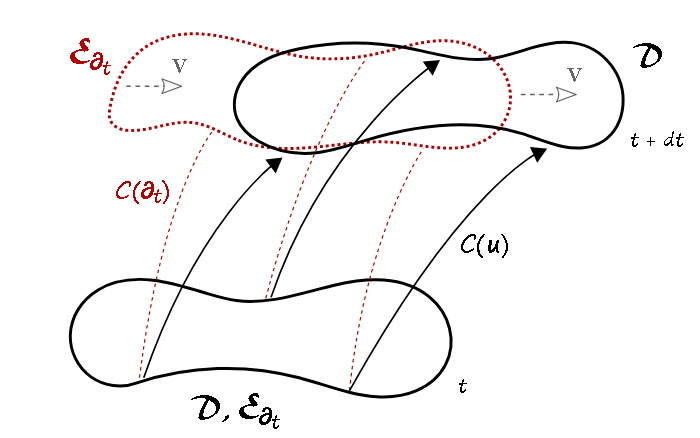
\includegraphics[scale=0.5]{domain_transportation.png}
\end{figure}

\textcolor{blue}{Aqui seguimos buchert, mas aplicamos para a congruencia de $n^\mu$}

This figure represents how the hypersurface $\Sigma$ is transported along the congruence $C(n)$, with $X^i=\text{const.}$. 
And is transported along the congruence $C(\partial_t)$, with $x^i=\text{const.}$, which coincides with $\Sigma$ at the time $t$. 
The domain undergoes a spatial motion, with velocity $\mathbf{\beta}$, in the coordinate basis $(t,x^i)$. Therefore $d/dt$ and $\int_\Sigma d^3x$ do not commute.

Consider a family of maps, $\bm{\Phi}_t=\mathbf{f}(t,\cdot)$, in order to change the coordinates $x^i$ to $X^i$,
\begin{equation}
	x^i = f^i(t,\mathbf{X}), \qquad d^3x = \text{det}\left(\frac{\partial \mathbf{f}(t,\mathbf{X})}{\partial \mathbf{X}}\right)d^3X = J(t,\mathbf{X})d^3X,
\end{equation}
while the domain transforms as, $\Sigma_x \rightarrow \Sigma_X = \mathbf{\Phi}^{-1}_t(\Sigma_x)$, the volume of the domain is then given by,
\begin{equation}
	V_\Sigma(t)=\int_{\Sigma_x}d^3x \sqrt{h(t,x^i)} \rightarrow V_\Sigma(t)=\int_{\Sigma_X}d^3X J(t,\mathbf{X})\sqrt{h(t,f^i(t,\mathbf{X}))}.
\end{equation}

The total derivative of coordinate time of the volume of domain,
\begin{align}
	\frac{d V_\Sigma}{dt} &= \int_{\Sigma_X}d^3X  \frac{d}{dt}\left(J(t,\mathbf{X})\sqrt{h(t,f^i(t,\mathbf{X}))}\right)=\int_{\Sigma_X}d^3x J^{-1} \frac{d}{dt}\left(J \sqrt{h}\right)=\\
	&=\int_{\Sigma_X}d^3x \left(\frac{d}{dt}\sqrt{h} - J \sqrt{h} \frac{d}{dt}\left(J^{-1}\right)\right)=\\
	&=\int_{\Sigma_X}d^3x \left(\partial_t\sqrt{h}-\beta^k\partial_k \sqrt{h} + J^{-1} \sqrt{h} \frac{d}{dt}J\right)
\end{align}
something useful here is,
\begin{align}
	\beta^i&=-\left.\frac{dx^i}{dt}\right|_{\mathbf{X}}=-\frac{d f^i(t,\mathbf{X})}{dt}=-\partial_t|_{\mathbf{X}} f^i(t,X) \Leftrightarrow \times \frac{d}{dX^i}\\
	\Leftrightarrow J \partial_i \beta^i &=- \partial_{X^i} \partial_t|_{\mathbf{X}} f^i(t,X) \Leftrightarrow \\
	\Leftrightarrow J \partial_i \beta^i &=- \partial_t|_{\mathbf{X}}  \partial_{X^i} f^i(t,X)\Leftrightarrow \\
	\Leftrightarrow J \partial_i \beta^i &=- \partial_t|_{\mathbf{X}}  J
\end{align}
\begin{align}
	\frac{d V_\Sigma}{dt} &=\int_{\Sigma_X}d^3x \left(\partial_t\sqrt{h}-\beta^k\partial_k \sqrt{h} - \sqrt{h} \partial_k \beta^k\right)\Leftrightarrow\\
	&=\int_{\Sigma_X}d^3x \left(\frac{1}{2}\sqrt{h} h^{ij}\partial_t h_{ij}-\frac{1}{2} h^{ij}\sqrt{h}\beta^k\partial_k h_{ij} - \sqrt{h} \partial_k \beta^k\right)=\\
	&=\int_{\Sigma_X}d^3x \sqrt{h} \left(\frac{1}{2} h^{ij}\partial_t h_{ij}-\frac{1}{2} h^{ij}\beta^k\partial_k h_{ij} - \partial_k \beta^k\right)=\\
	&=\int_{\Sigma_X}d^3x \sqrt{h} \left(\frac{1}{2} h^{ij}\partial_t h_{ij}-D_k\beta^k\right)
\end{align}
By the trace of Eq.(\ref{eqn:metric_evo_normal}) we see that,
\begin{equation}
	\frac{d V_\Sigma}{dt} =\int_{\Sigma_X}d^3x \sqrt{h}\left(NK\right)
\end{equation}
where $D_k$ is the three-covariant derivative.

Now diving by the volume we obtain,
\begin{equation}
	\frac{1}{V_\Sigma}\frac{d V_\Sigma}{dt} = \left\langle NK \right\rangle_{\Sigma}
	\label{eqn:general_volume_buchert}
\end{equation}

The commutative relation between the time derivative and the averaging operator is given by,
\begin{equation}
	\left[\frac{d}{dt}, \langle\cdot \rangle_{\Sigma}\right] S=\left\langle NKS\right\rangle_{\Sigma}-\left\langle NK \right\rangle_{\Sigma}\langle S\rangle_{\Sigma},
	\label{eqn:comoving_commutation_rule_buchert}
\end{equation}


\section{According to the Fluid Flow}